\documentclass[border=4pt]{standalone}
% Preámbulo común de las figuras. Cada figura es un documento standalone
% que se compila a SVG con scripts/build_figures.sh
\usepackage[utf8]{inputenc}
\usepackage{amsmath}
\usepackage{tikz}
\usepackage[american, siunitx]{circuitikz}
\usetikzlibrary{arrows.meta,calc,decorations.pathmorphing,patterns}
\tikzset{
  >={Stealth[length=2.2mm]},
  eje/.style={->, thin},
  hilo/.style={thick},
}
% Paleta común: tonos medios legibles sobre fondo claro
\definecolor{azul}{RGB}{31,94,168}
\definecolor{rojo}{RGB}{192,57,43}
\definecolor{verde}{RGB}{39,128,73}
\definecolor{naranja}{RGB}{211,120,30}
\definecolor{morado}{RGB}{125,60,152}

\begin{document}
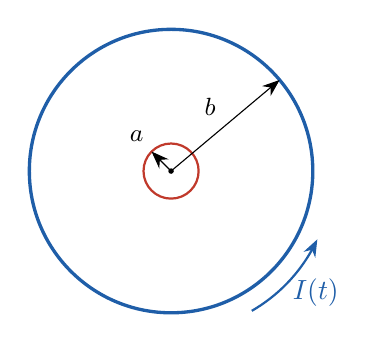
\begin{tikzpicture}[scale=1.0]
  \draw[very thick, azul] (0,0) circle (1.8);
  \draw[thick, rojo] (0,0) circle (0.35);
  \fill (0,0) circle (1pt);
  \draw[->] (0,0) -- (135:0.35);
  \node[font=\small] at (135:0.62) {$a$};
  \draw[->] (0,0) -- (40:1.8) node[midway, above left, font=\small]{$b$};
  \draw[->, thick, azul] (-60:2.05) arc[start angle=-60, end angle=-25, radius=2.05];
  \node[azul] at (-40:2.4) {$I(t)$};
\end{tikzpicture}
\end{document}
